\section{Results}
This section looks at the equations of motion and steady-state solutions of a \gls{qho}, both with and without feedback. The first subsection deals with a \gls{qho} which is measured continuously and without feedback, while the second subsection adds feedback into the scheme.
\subsection{Measurement Without Feedback}
Consider a \gls{qho} described by the Hamiltonian in Eq. \eqref{eq:hamiltonian} which is coupled to a thermal bath with temperature $T$. If the oscillator's position quadrature is also continuously measured, the evolution of the system can be described by the master equation in Eq. \eqref{eq:masterMeas} using the Lindblad operators mentioned in Sec. \ref{sec:mastereq}. We want to solve for the \gls{eom} for the first and second moments, when measuring for the position quadrature $\xop$. 

We start by looking at the first moments which are derived from
\begin{align}
    \dt\expval{\xop} &= \tr(\xop \dt \dmatrix),\\
    \dt\expval{\pop} &= \tr(\pop \dt \dmatrix).
\end{align}
Inserting the master equation in Eq. \eqref{eq:masterMeas} we find 
\begin{align}
    \dt\expval{\xop} &= -\frac{\gamma}{2} \expval{\xop} - \frac{1}{m} \expval{\pop},\\
    \dt\expval{\pop} &= -\frac{\gamma}{2} \expval{\pop} + m\omega^2 \expval{x}.
\end{align}
Then when solving for the steady state we find 
\begin{equation}
    \expval{\xop} = \expval{\pop} = 0. \label{eq:xp0}
\end{equation}
This result also confirms the intuition that for a harmonic oscillator, the system has a steady state around the origin. 

It is also important to investigate the stability of the system. That is, if and when the system, in the long time limit, will end up in a steady state, and that the steady state is stable to small perturbations. To check for stability we can rewrite the equation as an eigenvalue problem and solve for the eigenvalues.
\begin{equation}
    \dt 
    \begin{pmatrix}
        \expval{\xop}\\
        \expval{\pop}    
    \end{pmatrix}
    = \mathcal{M}
    \begin{pmatrix}
        \expval{\xop}\\
        \expval{\pop} 
    \end{pmatrix},
\end{equation}
for the matrix
\begin{equation}
    \mathcal{M} = \begin{pmatrix}
        -\gamma/2 & -1/m \\
        m\omega^2 & -\gamma/2
    \end{pmatrix}.
\end{equation}
The eigenvalues of $\mathcal{M}$ are 
\begin{align}
    \lambda_1 &= -\frac{\gamma}{2} - i\omega,\\
    \lambda_2 &= -\frac{\gamma}{2} + i\omega.
\end{align}
Since the real part of the eigenvalues are negative the system is stable. This is because we can write the time-dependant solutions of the dynamical equations as an exponential with the eigenvalues while the coefficients are chosen by the initial condition, the value of the eigenvalues will determine the behaviour of the system. The consequence of the real part of the eigenvalue being negative is that it will make the function decay with time and is thus considered stable. If both eigenvalues are negative the system will decay no matter what the initial conditions are since both terms in the solution will decay. Positive eigenvalues on the other hand will correspond to the system growing with time and will thus be unstable. When one of the eigenvalues is positive and the other is negative the stability of the system will be determined by the initial conditions. That is, the initial condition will determine which eigenvalue will dominate the solution.

We now solve the \gls{eom} for the second moments using the same method of inserting the master equation, derived from
\begin{align}
    \dt\expval{\xop^2} &= \tr(\xop^2 \dt \dmatrix)\label{eq:x2}, \\
    \dt\expval{\pop^2} &= \tr(\pop^2 \dt \dmatrix)\label{eq:p2},\\
    \dt\expval{\acomm{\xop}{\pop}} &= \tr(\acomm{\xop}{\pop} \dt \dmatrix). \label{eq:xp}
\end{align}
The choice of looking at the second moments has to do with their relation to the variance and thus the fluctuations of the system. These fluctuations are then related to the energy contained in the oscillator, as the expectation value of the Hamiltonian. When looking at feedback control one application is to minimize the energy in the oscillator and, which is thus also an argument for looking at the second moments. Inserting the quantum master equation in Eq. \eqref{eq:masterMeas} and solving Eqs. \eqref{eq:x2} to \eqref{eq:xp} yields the following \gls{eom}
\begin{align}
    \dt\expval{\xop^2} &= - \gamma \expval{\xop^2} - \frac{1}{m}\expval{\acomm{\xop}{\pop}} + \frac{\gamma \hbar}{m\omega}(\nbar + 1/2),\\
    \dt\expval{\pop^2} &= -\gamma \expval{\pop^2} + m\omega^2 \expval{\acomm{\xop}{\pop}} + \gamma m \omega\hbar (\nbar + 1/2) + \lambda \hbar^2,\\
    \dt\expval{\acomm{\xop}{\pop}} &= -\gamma \expval{\acomm{\xop}{\pop}} + 2 m \omega^2 \expval{\xop^2} - \frac{2}{m} \expval{\pop^2}.
\end{align}
For more detailed calculations, see App. \ref{app:eom}. Performing a change of variable to make the equations dimensionless
\begin{equation}
    \tilde{x} = \sqrt{\frac{m\omega}{\hbar}} x \quad \text{and} \quad \tilde{p} = \sqrt{\frac{1}{m \omega \hbar}} p ,
\end{equation}
we can solve for the steady state, by setting the time derivative to zero. Introducing the quality factor $Q = \omega / \gamma$ we obtain the steady-state solutions
\begin{align}
    \expval{\tilde{x}^2}_\mathrm{ss} &= (\nbar + 1/2) + \frac{\lambda \hbar}{m \omega^2} \frac{2 Q^3}{4Q^2 + 1}, \label{eq:x2ss}\\
    \expval{\tilde{p}^2}_\mathrm{ss} &= (\nbar + 1/2) + \frac{\lambda \hbar}{m \omega^2} \left( Q - \frac{2Q^3}{4Q^2 + 1} \right) \label{eq:p2ss},
\end{align}
One aspect of the steady-state solutions is that both equations have identical terms capturing the thermal aspect of the fluctuations. Without measurement, the steady states are only thermal, which is to be expected. When calculating the energy of the steady state the complicated fraction above cancels, and we are left with a purely linear term in the quality factor.
\begin{equation}
    E_\mathrm{ss} = \expval{\tilde{H}}_\mathrm{ss} = \frac{\hbar \omega}{2} \left( \expval{\tilde{p}^2}_\text{ss} + \expval{\tilde{x}^2}_\text{ss} \right) = \hbar\omega (\nbar + 1/2)+ \frac{\lambda \hbar^2}{2 m\omega} Q
    \label{eq:ess}
\end{equation}
To simplify plotting we might perform the change of variable
\begin{equation}
    \tilde{E} =\frac{E}{\hbar\omega}, \quad \Lambda = \frac{\lambda \hbar}{m \omega^2}.
\end{equation}

\begin{figure}
    \centering
    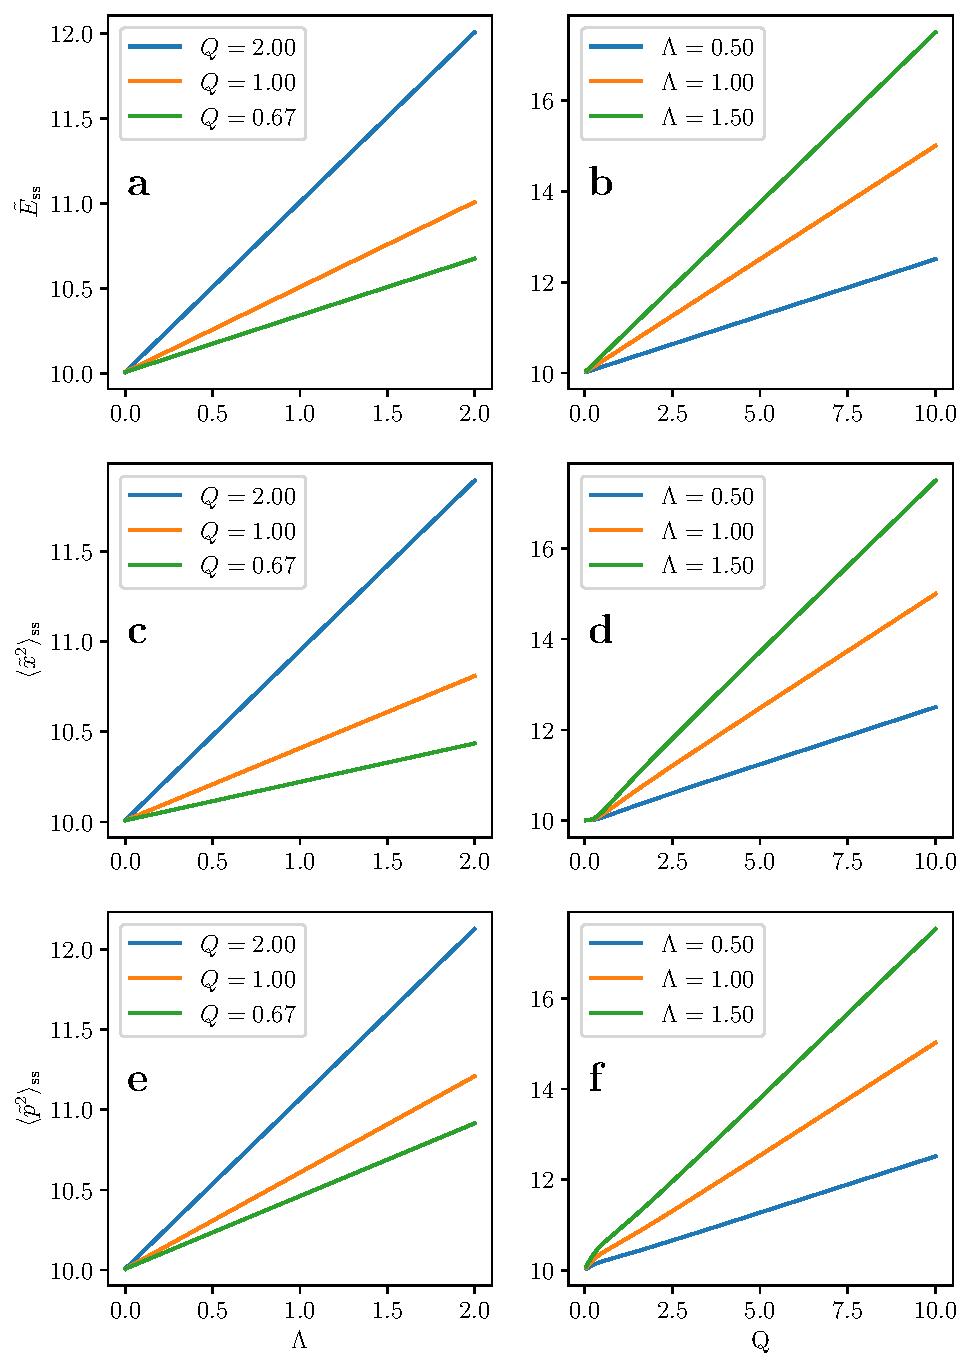
\includegraphics[width=\textwidth]{measurement_result.pdf}
    \caption{ \small The top panels show Eq. \eqref{eq:ess}, the middle panels show Eq. \eqref{eq:x2ss} and the bottom panels show Eq. \eqref{eq:p2ss}. All plots use the parameters $k_\mathrm{B}T = 10$ and $\omega = \hbar = 1$. The left panels are plotted against $\lambda / \omega$ and with three different values for $Q$, while the right panels are plotted against $Q$ and three different values of $\lambda$. }
    \label{fig:steady_state}
\end{figure}

Looking at panels \textbf{a} and \textbf{b} in Fig. \ref{fig:steady_state} one can see that a stronger measurement correlates to the system's steady state increasing in energy, as does it for an increasing quality factor. Both also affect the system linearly. Thus, by continuously measuring the system we add energy into it, which make the steady state higher in energy than what the thermal effects from the bath would otherwise place it. That is, if we do not perform any measurement the system would be stable at around $\nbar + 1/2$ which for the parameters used here would give $E_\text{ss} \approx 10\hbar\omega$.

In panels \textbf{d} and \textbf{f} we can see that there is some non-linear behaviour near $Q = 0$. However, due to the approximations made in Sec. \ref{sec:open} we cannot trust the results in the region of a low quality factor. This is because this regime has a relatively high coupling to the environment, and thus the excitations in the environment might not decay fast enough and therefore affect the oscillator. Panels \textbf{c} and \textbf{e} show the linear dependence on $\Lambda$ for the second moments.


Eq. \eqref{eq:xp0} together with Eqs. \eqref{eq:x2ss} and \eqref{eq:p2ss} also shows that the variance of the system is only dependent on the second moments, since
\begin{equation}
    \sigma^2_{\hat{A}} = \expval{\hat{A}^2} - \expval{\hat{A}}^2
\end{equation}
for an operator $\hat{A}$. It is also an easy calculation then to show that for temperature $T=0$ and without measurement we have equality in the Heisenberg uncertainty relation, $\sigma_{\xop} \sigma_{\pop} = \hbar/2$, justifying the accuracy of the results, and the approximations made in the derivation of the master equation.

\subsection{Feedback}
We now consider a feedback mechanism on the oscillator described by Eq. \eqref{eq:masterFeed} which is a linear feedback scheme. Solving for the first moments' \gls{eom} we find 
\begin{align}
    \dt\expval{\xop} &= - \left(\frac{\gamma}{2} + \frac{2 \im{f}}{\sqrt{2 m \omega \hbar}} \right)\expval{\xop} - \frac{1}{m} \expval{\pop},\\
    \dt\expval{\pop} &= -\frac{\gamma}{2}\expval{\pop} + \left(\re{f} \sqrt{\frac{2 m \omega}{\hbar}} + m \omega^2 \right) \expval{\xop}.
\end{align}
We see that when measuring $\xop$ the feedback terms enter the equations on the position quadrature. A real $f$, $\im{f} = 0$, removes the feedback for the equation of the position, while an imaginary $f$, $\re{f} = 0$, removes the feedback for the equation of the momentum. The equations are still coupled however, since the position is dependent on the momentum and vice versa. Setting $f = 0$, yields the previous result. The steady state solutions for this system are $\expval{\xop} = \expval{\pop} = 0$.

We notice that it is possible to remove $\expval{\xop}$ from the equations, so the system reduces to 
\begin{align}
    \dt\expval{\xop} &= - \frac{1}{m} \expval{\pop},\\
    \dt\expval{\pop} &= -\frac{\gamma}{2} \expval{\pop},
\end{align}
by choosing $f$ such that
\begin{equation}
    \re{f} = - \sqrt{\frac{m \omega^3 \hbar}{2}} \quad \text{and} \quad \im{f} = -\frac{\gamma\sqrt{m\omega\hbar}}{2\sqrt{2}} \label{eq:reFimF_toZero},
\end{equation}
which has a steady-state solution for $\expval{\pop} = 0$ and any $\expval{\xop}$. We find the eigenvalues for this choice of $f$ to be $\varepsilon_- = -\gamma /2$ and $\varepsilon_+ = 0$. This choice of $f$ removes all the oscillatory behaviour from the system, which can be seen by the eigenvalues being real. This puts it in the region of being overdamped by the choice of $f$. Since one of the eigenvalues are zero, the system is also  one dimensional, which is reasonable as the choice of $f$ is such that the first moments' dynamics are independent of the position average.

To check for stability of the first moments, we first perform the change of variable
\begin{equation}
    \tilde{f} = \frac{f}{\omega \sqrt{m \omega \hbar}},
\end{equation}
and rewrite the equations as an eigenvalue problem with matrix
\begin{equation}
    \mathcal{M} = 
    \begin{pmatrix}
        - \left(\frac{\gamma}{2} + \sqrt{2} \im{\tilde{f}} \omega \right) & - \frac{1}{m} \\
        m \omega^2\left(\sqrt{2}\re{\tilde{f}} + 1\right) & -\frac{\gamma}{2}
    \end{pmatrix}, \label{eq:matrixM}
\end{equation}
which has eigenvalues
\begin{equation}
    \frac{\varepsilon\pm}{\omega} = \sqrt{\frac{\im{\tilde{f}}^2}{2} - \sqrt{2} \re{\tilde{f}} - 1 } - \frac{\im{\tilde{f}}}{ \sqrt{2}} - \frac{1}{2Q} \label{eq:eigenvalueFirstMomenta}
\end{equation}


\begin{figure}
    \centering
    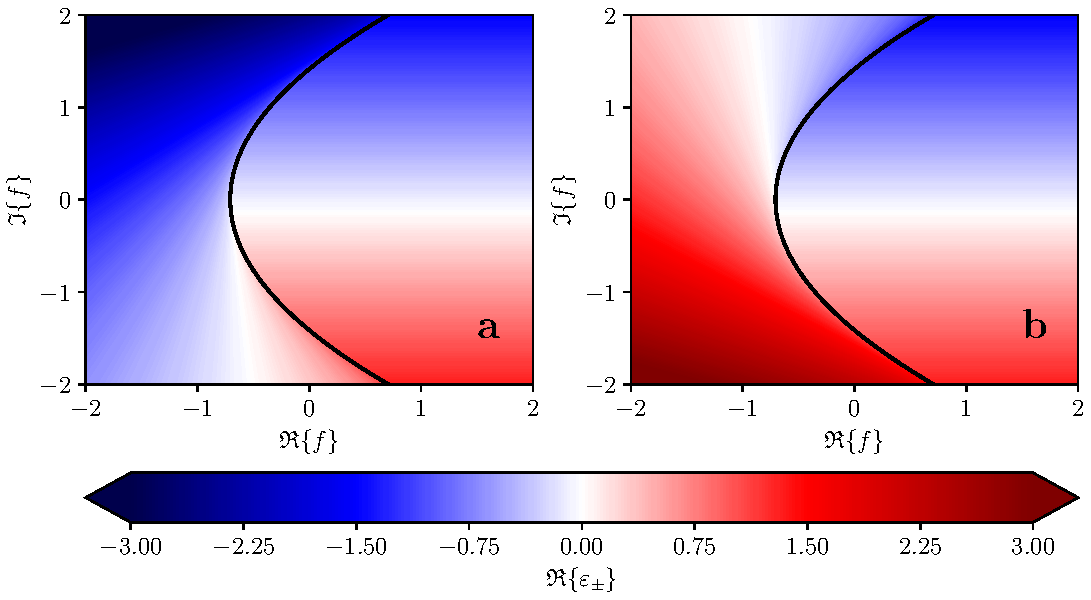
\includegraphics[width=\textwidth]{figures/eigenvalueFirstMomenta.pdf}
    \caption{\small Eq. \eqref{eq:eigenvalueFirstMomenta} plotted as a contour plot against the real and imaginary part of $f$. The parameter used is $Q = 10$. Panel \textbf{a} shows $\re{\varepsilon_-/\omega}$ and panel \textbf{b} shows $\re{\varepsilon_+\omega}$. The parabola that can be seen in both panels is the points where the first square root in Eq. \eqref{eq:eigenvalueFirstMomenta} is zero. Thus, points to the left of this parabola are real, while points to the right are complex, only the real part is plotted, however.}
    \label{fig:eigenvalueFirstMomenta}
\end{figure}

Looking at Fig. \ref{fig:eigenvalueFirstMomenta} we can see that $\re{\varepsilon_- / \omega}$ is mostly negative while $\re{\varepsilon_+ / \omega§}$ is mostly positive for the parameters used in the region closest to the origin. The only part where both eigenvalues are negative is in top right region of the figures. That is, the region where $\im{\tilde{f}} > 0$ and $\re{\tilde{f}} \gtrapprox -0.7$. The reason for the approximation is that it is not an analytical result, but instead apparent from looking at panel \textbf{b}, where we can see that line where the eigenvalue is zero, and has a slant and is not vertical. 

It is important to remember that we can solve the dynamics of the system as exponentials with the eigenvalues, and some coefficients determined by the initial conditions. For an equation on the form
\begin{equation}
    \dt \vec{x}(t) = \mathcal{A}\vec{x}(t),
\end{equation}
with a vector $\vec{x}$ and a diagonalizable matrix $\mathcal{A}$, we can write the solution as
\begin{equation}
    \vec{x}(t) = \sum_i c_i e^{\lambda_i t} \vec{u}_i,
\end{equation}
where $\lambda_i$ is the i'th eigenvalue, and $\vec{u}_i$ is the i'th eigenvector. It is apparent that in the case when $c_i \neq 0$ for all $i$, the eigenvalues $\lambda_i$, must have a negative real part for the system to be stable, as otherwise one of the terms in the sum would diverge. 

Another thing to note is that the eigenvalues are complex to the right of the black parabola in the figure, and thus the solution will have oscillatory motion in this region.

Solving for the \gls{eom} for the second moments we obtain
\begin{align}
    \dt \expval{x^2} &= -\left(\gamma + \frac{4\im{f}}{\sqrt{2 m \omega \hbar}}\right) \expval{x^2} - \frac{1}{m} \expval{\acomm{x}{p}} + \frac{\gamma \hbar}{m \omega} (\nbar + 1/2) \nonumber\label{eq:x2Feedback} \\
    &\qquad - \frac{1}{4\lambda m \omega \hbar} \re{f}^2,\\
    \dt \expval{p^2} &=  -\gamma \expval{p^2} + \left( m\omega^2 + \re{f} \sqrt{\frac{2m \omega}{\hbar}} \right)\expval{\acomm{x}{p}} + \gamma m \omega \hbar (\nbar + 1/2) \nonumber \\
    &\qquad+ \lambda \hbar^2 + \frac{m \omega}{4 \lambda \hbar}\re{f}^2,\label{eq:p2Feedback} \\
    \dt \expval{\acomm{x}{p}} &= -\left(\gamma + \frac{2\im{f}}{\sqrt{2m \omega \hbar}}  \right)\expval{\acomm{x}{p}} + \left(2 m \omega^2 + 2 \sqrt{\frac{2 m \omega}{\hbar}}\re{f} \right) \expval{x^2} - \frac{2}{m} \expval{p^2}\nonumber\\ 
    &\qquad - \frac{\re{f} \im{f}}{2 \lambda \hbar}.\label{eq:xpFeedback}
\end{align}
We can solve for the steady state by first rewriting the system of equations to a matrix equation $\dt X = \mathcal{A} X + \mathcal{B}$ where
\begin{equation}
    X =
    \begin{pmatrix}
        \expval{\xop^2}\\
        \expval{\pop^2}\\
        \expval{\acomm{\xop}{\pop}}    
    \end{pmatrix}, \quad
    \mathcal{A} = \begin{pmatrix}
        -\left(\gamma + \frac{4\im{f}}{\sqrt{2 m \omega \hbar}}\right) & 0 & -\frac{1}{m} \\
        0 & -\gamma & m\omega^2 + \re{f} \sqrt{\frac{2m \omega}{\hbar}} \\
        2 m \omega^2 + 2 \sqrt{\frac{2 m \omega}{\hbar}}\re{f} & -\frac{2}{m} & -\left(\gamma +\frac{2\im{f}}{\sqrt{2m \omega \hbar}}\right) \label{eq:matrixA}
    \end{pmatrix}
\end{equation}
and
\begin{equation}
    \mathcal{B} = 
    \begin{pmatrix}
        \frac{\gamma \hbar}{m \omega} (\nbar + 1/2) - \frac{\re{f}^2}{4\lambda m \omega \hbar}\\
        \gamma m \omega \hbar (\nbar + 1/2) + \lambda \hbar^2 +\frac{m \omega \re{f}^2}{4 \lambda \hbar}\\
        -\frac{\re{f} \im{f}}{2 \lambda \hbar}
    \end{pmatrix}.
\end{equation}
We notice the addition of a constant term in all three equations corresponding to the noise of the feedback, that is, all these terms comes from the second feedback term in Eq. \eqref{eq:masterFeed}. Furthermore, we see that a driving feedback term has entered all three equations on the position quadrature and the anticommutator, which contains $\xop$. It's worth noting the similarities of the terms between equations.

To obtain the steady-state solutions we solve $X_\text{ss} = - \mathcal{A}^{-1} \mathcal{B}$. To simplify this we perform the same change of variables as before. The full analytical solutions are not shown here due to the length of the equations. It would also be possible to solve the matrix equation numerically. To get an understanding of the steady-state solution we look at figures generated by the solution.

\begin{figure}[t]
    \centering
    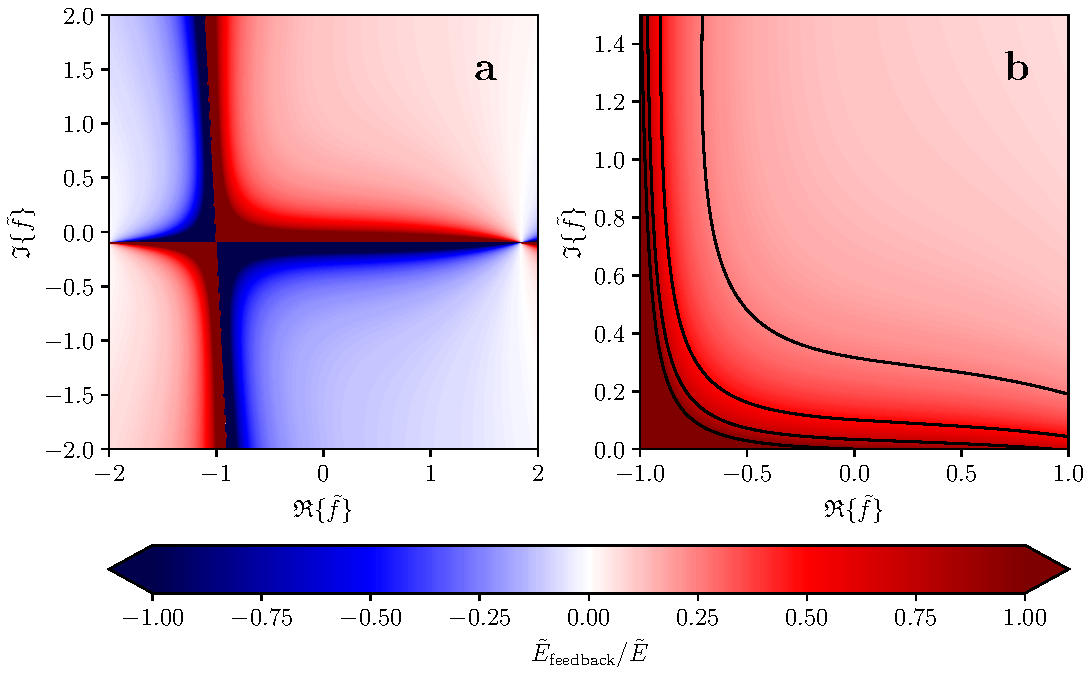
\includegraphics[width=\textwidth]{figures/energyFeedbackRatio.pdf}
    \caption{\small The ratio between the energy with feedback and without plotted as a contour plot against $\re{\tilde{f}}$ and $\im{\tilde{f}}$. The parameters used are $k_\text{B}T = 10 \hbar\omega$, $Q = 10$, $\Lambda = 2$. Panel \textbf{a} shows a large variation of the parameters. There are divergences in the plot which almost follow a $\left(\re{\tilde{f}} + 1 \right)\im{\tilde{f}} = 1$ curve. Panel \textbf{b} is a zoomed in version of panel \textbf{a} and shows the behaviour of the system in a region where the ratio always is positive. The contour lines in panel \textbf{b} are placed at the values of the tick marks in the colourbar.}
    \label{fig:energyFeedbackRatio}
\end{figure}
In Fig. \ref{fig:energyFeedbackRatio} we can see the effect the feedback has on the energy of the system. Looking at panel \textbf{a} we can see areas which are negative. If the energy of the system without measurement is constant, it must be the feedback energy that becomes negative. In the way we have set up the model, a negative energy is unreasonable, since a temperature of $T=0$ would correspond to $E =\hbar\omega( 1/2 + \Lambda Q/2)$, which without measurement would mean an energy of $E = \hbar\omega/2$. A possible explantation for the negative energy is that the specific feedback that give rise to this is affecting the system in such a way that at least one of our assumptions is no longer accurate. This could, for example, be that the system no longer have a physical steady state. Another reason might be that the Markovian approximation no longer holds.

Another interesing aspect of Fig. \ref{fig:energyFeedbackRatio} is that when looking at panel \textbf{b} in conjunction with Eq. \eqref{eq:ess} is that it is possible to cool the system to a lower energy than the thermal energy. Using the same parameters in Eq. \eqref{eq:ess} as are used in the figure we find that the thermal energy is half of the total energy in the system without feedback, and looking at the figure we see that there exist a region which has a ratio of less than $0.5$.

If one tweaks the parameters used in Fig. \ref{fig:energyFeedbackRatio} the general form of the plot remains the same, with some differences. The measurement strength $\Lambda$ does not affect the plot much, but it does however increase the energy, the contour lines in panel \textbf{b} remains almost the same. Thus, the same feedback would remove the same proportion of energy, it does however mean that a larger proportion need to be removed before cooling below the thermal equilibrium. Similarly, changing $k_\text{B}T$ does not dramatically change how the plot looks, but it does increase the energy of the system as well. However, since the thermal energy now constitute a larger part of the total energy of the system, a smaller feedback parameter is needed to cool the system below the thermal equilibrium. The quality factor $Q$ however, changes the plot quite a lot, decreasing the spacing between the contour lines and increasing the efficiency of the cooling.

\begin{figure}[t]
    \centering
    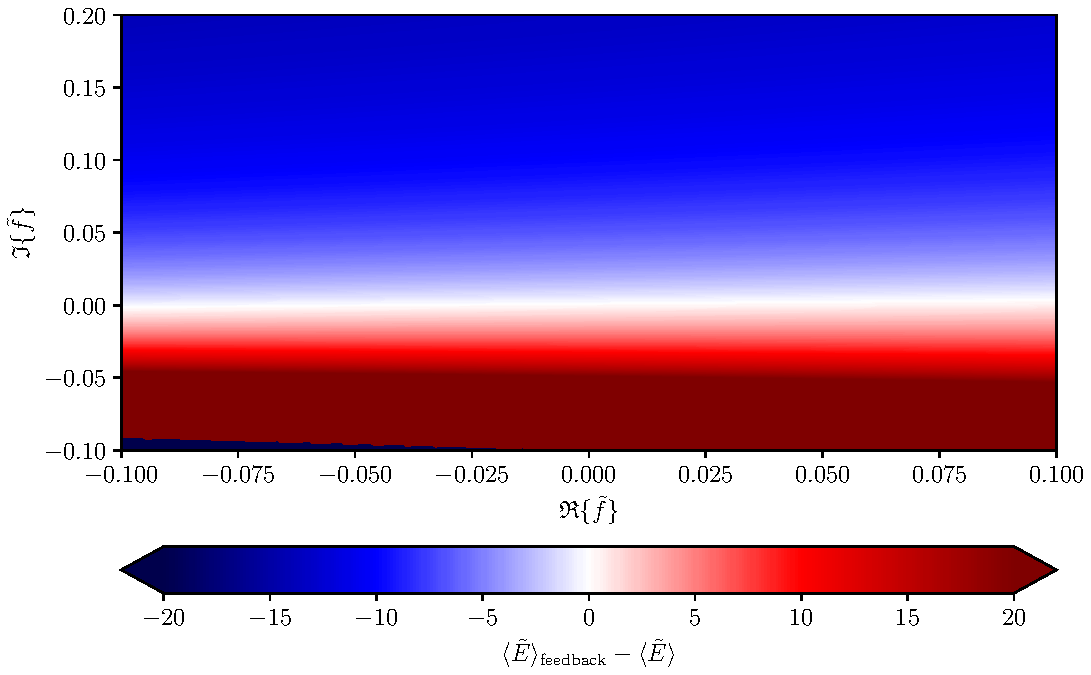
\includegraphics[width=\textwidth]{figures/energyFeedbackDifference.pdf}
    \caption{\small The difference between the energy of the system with feedback plotted and the energy without feedback plotteda against $\re{\tilde{f}}$ and $\im{\tilde{f}}$. The parameters used are $k_\text{B}T = 10 \hbar\omega$, $Q = 10$, $\Lambda = 2$. The plot is done in a small region around the origin, thus showing the effect a small feedback has on the system. The spacing between the contour lines is $2$ and the solid lines is at $0$.}
    \label{fig:energyFeedbackDifference}
\end{figure}

Using the parameters as in Fig. \ref{fig:energyFeedbackDifference} the energy without feedback is $\expval{\tilde{E}} \approx 20$ with the thermal part accounting for around $10$ of that. Looking at Fig. \ref{fig:energyFeedbackDifference} it is possible to see that even with a relatively low amount of feedback the system will be cooled to some degree. However, depending on how the feedback is applied it can also make the energy in the system diverge which can be seen for $\im{\tilde{f}} < 0$.

Due to the uncertainty relation and the canonical commutation relation $\xop^2$, $\pop^2$, and $\acomm{\xop}{\pop}$ are not independent \cite{Simon:1994}. This has the consequence that the stability analysis cannot be performed with $\mathcal{A}$ and $\mathcal{B}$. Instead, we rewrite $X$ as a quantum variance matrix \cite{Simon:1994}, and write Eqs. \eqref{eq:x2Feedback} to \eqref{eq:xpFeedback} as a Lyapunov equation
\begin{equation}
    \dt S = \mathcal{M} S + S \mathcal{M}^T  + \mathcal{C} = 0
\end{equation}
where 
\begin{align}
    S &= 
    \begin{pmatrix}
    \expval{\xop^2} & \expval{\acomm{\xop}{\pop}}/2\\
    \expval{\acomm{\xop}{\pop}}/2 & \expval{\pop^2}    
    \end{pmatrix},
    \\
    \mathcal{C} &=
    \begin{pmatrix}
        \frac{\gamma \hbar}{m \omega} (\nbar + 1/2) - \frac{\re{f}^2}{4\lambda m \omega \hbar} & -\frac{\re{f} \im{f}}{4 \lambda \hbar}\\
        -\frac{\re{f} \im{f}}{4 \lambda \hbar} & \gamma m \omega \hbar (\nbar + 1/2) + \lambda \hbar^2 +\frac{m \omega \re{f}^2}{4 \lambda \hbar}
    \end{pmatrix},
\end{align}
and $\mathcal{M}$ is the same matrix as in Eq. \eqref{eq:matrixM}, but using $f$ instead of $\tilde{f}$. $S$ has unique steady-state solutions if the real part of the eigenvalues of $\mathcal{M}$ are negative \cite{Purkayastha:2022}. We can therefore refer back to Eq. \eqref{eq:eigenvalueFirstMomenta} and Fig. \ref{fig:eigenvalueFirstMomenta} to see the stability of the system. In conjunction with Fig. \ref{fig:energyFeedbackRatio} and \ref{fig:energyFeedbackDifference} we can see that the system is stable in the region where we cool the system. Thus, it is not only possible to cool the system, but the system is also stable. We can therefore see that this type of feedback mechanism is a valid way to cool a \gls{qho}.